\chapter{行波管的特性参量及其测量} \label{ch:11}
为了检查行波管的质量,我们需要对它的特性参量进行考核。本章将介绍行波管的一般特性、参量及其测量方法。

行波管的参量都是与一定的频率相联系的。首先,我们介绍带宽和工作频率范围这样两个不同的概念。


行波管的带宽是指当管子的工作状态不变,其特定参量均能满足要求的一段频率间隔。而工作频率范围是指借助于调整行波管的工作状态,使其特定参量均能满足要求的一段频率间隔。所谓特定参量,各种行波管不尽一致,一般指功率、增益、噪声系数、驻波比等。可见,带宽与工作频率范围的区别就在于工作状态能否调整。以某行波管为例,它的工作频率范围是3800兆赫\textasciitilde4200兆赫(即工作频带宽度为400兆赫);当该行波管使用于微波接力通信中的某个具体波道上时,由于波道带宽只有20兆赫(中心频率$ \pm 10 $兆赫),因而工作状态就可按照这20兆赫内的最佳性能来调整,不必考虑整个工作频率范围以内的其它波道了


带宽一般远小于工作频率范围,这是微波接力通信用行波管的重要特点之一。由此,又可以引伸出来参量上的一系列特点。
\section{ 输入输出特性、增益、功率}
在一定的工作状态下,行波管的输出功率随输入功率而变化的特性,叫做行波管的输入输出特性,又叫转移特性,如图\ref{ch11-1}所示。

\begin{figure}[phtb]
	\centering
	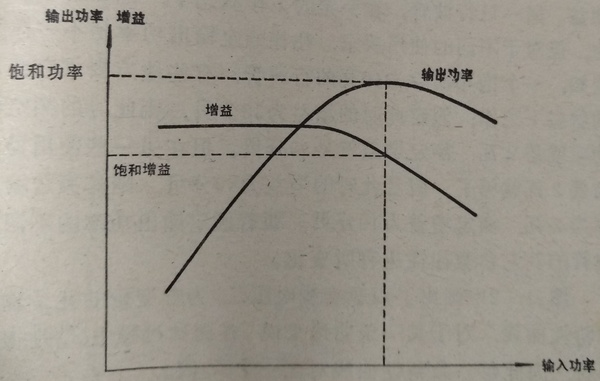
\includegraphics[width=0.6\linewidth]{figure/ch11-1}
	\caption{ 行波管的输入输出特性}
	\label{ch11-1}
\end{figure}

图\ref{ch11-1}中,纵坐标是行波管的增益$ G $,它是输出功率$ P_2 $与输入功率$ P_1 $的比,一般用分贝(dB)表示:
\begin{equation} \label{eq:11-1}
	G = 10\lg \frac{P_2}{P_1}\,\textrm{(dB)}
\end{equation}
从图中可以看出:当输入功率较小时,输出功率和输入功率之间具有线性的关系,我们把它叫做小信号增益,有时也叫线性增益;当输入功率较大时,输入功率和输出功率之间关系就不是线性的了,此时输出功率的增加比较缓慢,同时,增益也逐渐降低。在输入功率由小到大的变化过程中,输出功率存在一个最大值,这时的输出功率叫做饱和功率,这时的增益叫饱和增益。通常饱和增益要比小信号增益小6分贝左右。


有时要求行波管工作在规定的输入功率(叫做额定输入功率)条件下,此时输出功率就叫做额定输出功率,增益叫额定增益。同一只行波管,在一定的工作状态下,饱和功率是一定的,但对于不同的使用要求,往往额定输出功率是不一样的。例如:一个饱和功率为10瓦的行波管,有些地方要求它在8瓦的状态下工作,假定此时的增益为38分贝,则此时的额定输出功率就是8瓦,额定增益就是38分贝。但在另一些使用场合,需要2瓦就够了,假若此时的增益为40分贝,则其额定输出功率为2瓦,额定增益为40分贝。随着额定输出功率的不同,行波管的其它参数往往也有所变化。


图\ref{ch11-2}中画出了以螺旋线电压$ U_H $为参变量的几条输入输出特性曲线,对于某一条曲线来说,在测试过程中$ U_H $是保持不变的,因此每一条特性曲线对应一个$ U_H $值。


\begin{figure}[phtb]
	\centering
	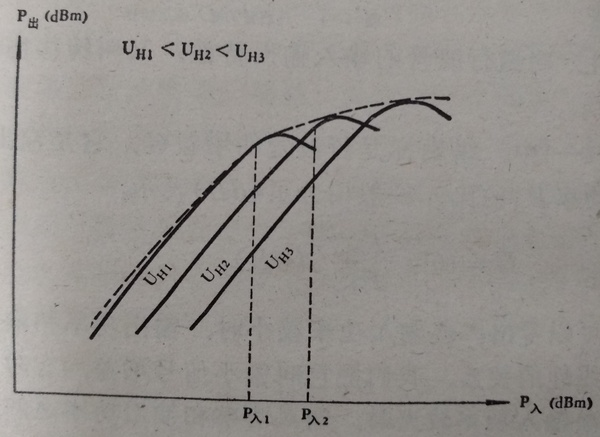
\includegraphics[width=0.6\linewidth]{figure/ch11-2}
	\caption{输入输出特性随螺旋线电压的变化}
	\label{ch11-2}
\end{figure}

如果我们在测试输入输出特性时,并不保持$ U_H $不变,而是每当输入功率改变时,用调节螺旋线电压$ U_H $的办法使其输出功率调到最大,那么,此时的输入输出特性就如图\ref{ch11-2}中虚线所示。


当输入功率为$ P_{\textrm{入}1} $时,螺旋线电压为$ U_{H1} $就比为$ U_{H2} $时的增益高,输出功率大,此时同步电压为$  U_{H1} $。当输入功率为$ P_{\textrm{入}2} $时,则螺旋线电压为$ U_{H2} $时输出最大,增益最高,此时同步电压为$ U_{H2} $。输入功率改变时,螺旋线电压也跟着改变,始终保持同步,这样获得的增益叫最佳增益,这样获得的饱和功率、饱和增益叫最佳饱和功率、最佳饱和增益。


行波管的增益随工作状态的变化而变化。如果电子注电流是一定的,则增益不仅随输入功率变化,而且还随螺旋线电压的变化而变化。我们把输入功率一定时,增益随螺旋线电压变化的特性叫做行波管的同步特性,如图\ref{ch11-3}所示。

\begin{figure}[phtb]
	\centering
	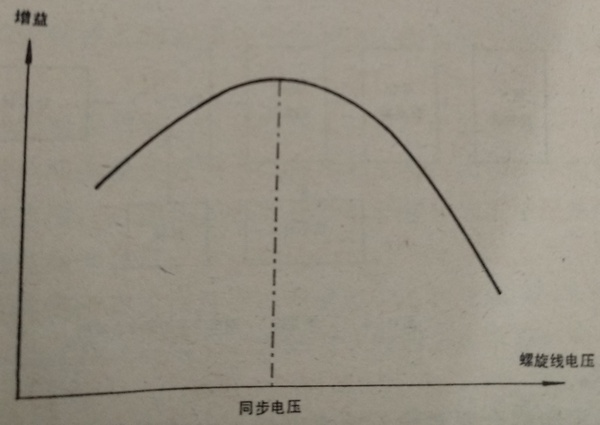
\includegraphics[width=0.6\linewidth]{figure/ch11-3}
	\caption{同步特性}
	\label{ch11-3}
\end{figure}

关于同步特性,已经做过介绍,读者可以回忆一下。

前面谈到输入输出特性、同步特性、功率(额定功率、饱和功率、最佳饱和功率)、增益(小信号增益、额定增益、饱和增益、最佳增益,最佳饱和增益)等,测量这些特性或参量、实际上就是测量行波管的输入、输出功率,然后经过一些计算即可得到相应的参量。功率测量的原理方框图如图\ref{ch11-4}所示

\begin{figure}[phtb]
	\centering
	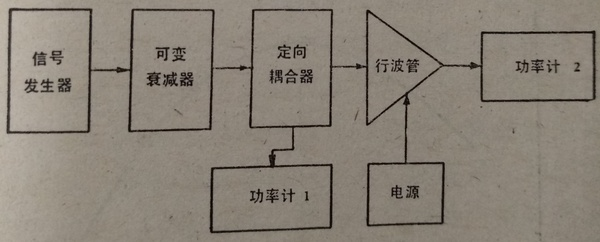
\includegraphics[width=0.6\linewidth]{figure/ch11-4}
	\caption{测量输入、输出功率的原理方框图}
	\label{ch11-4}
\end{figure}

定向耦合器对输入功率取样,由功率计1测出输入功率功率计2则用来测量输出功率。若功率计2量程不够,可用定向合器或衰减器(或两者都用)来扩大功率计2的量程。
\section{增益频率特性}
行波管增益随频率的变化我们可以画成曲线,称为增益频事特性曲线,如图\ref{ch11-5}所示。在通信中,希望这个变化越小越好。衡量这个特性的指标有三个:增益的均匀性、增益脉动和增益斜率。

\begin{figure}[phtb]
	\centering
	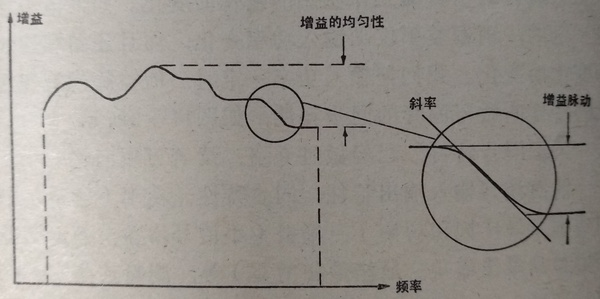
\includegraphics[width=0.6\linewidth]{figure/ch11-5}
	\caption{增益频率特性曲线}
	\label{ch11-5}
\end{figure}

增益的均匀性被定义为:行波管在某一工作状态下,在整个工作频率范围内最大增益与最小增益之差。通常用于衡量整个工作频率范围内工作状态不可调的行波管(如卫星通信中的行波管)增益频率特性。


增益脉动是行波管在某一工作状态下,在一定频率范围(此范围小于行波管的整个工作频带)内的最大增益与最小增益之差。


增益斜率则是增益频率特性曲线上某一频率点下的斜率用分贝/兆赫表示。


在地面微波接力通信设备中,由于行波管实际上是工作在某一个特定的波道中的,而每个波道的频带较窄,故常用增益脉动、增益斜率来考察行波管的增益频率特性。


增益频率特性常用扫频的方法测量,其测量原理方框图如图\ref{ch10-6}所示。

\begin{figure}[phtb]
	\centering
	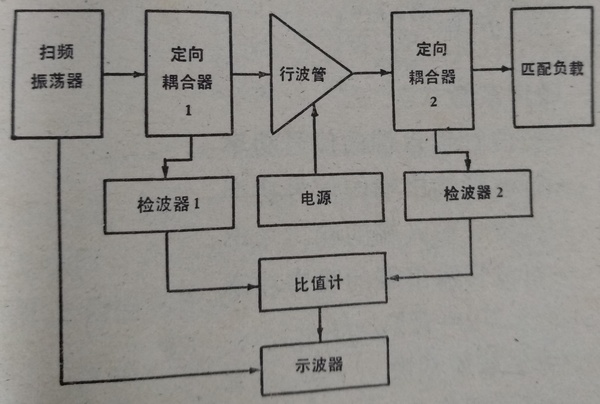
\includegraphics[width=0.6\linewidth]{figure/ch11-6}
	\caption{测量输入、输出功率的原理方框图}
	\label{ch11-6}
\end{figure}

定向耦合器1、2分别对行波管的输入、输出信号取样经检波后,它们就代表了输入、输出功率的大小。若定向耦合器1与2、检波器1与2完全对称,则两个检波器输出之比就代表了输出功率与输入功率之比,即反映了行波管的增益。所以,比值计的输出就反映了增益的大小,可在示波器上显示也可用$ X—Y $记录仪记录。


扫频振荡器能给出在规定频率范围内频率连续可变的信号,要求输出稳定,一般都有稳幅装置。

\section{噪声系数与基带噪声}
\subsection{噪声系数}


与任何放大器一样,行波管在放大信号的同时,其本身还产生噪声。通常用噪声系数来衡量这个噪声的大小,它的定义是:
\begin{equation} \label{eq:11-2}
	F = \frac{S_1/N_1}{S_2/N_2}
\end{equation}

式中:

$ F $—噪声系数


$ S_1 $—行波管输入端的信号功率


$ S_2 $—行波管输出端的信号功率


$ N_1 $—行波管输入端的噪声功率


$ N_2 $—行波管输出端的噪声功率

又:
\begin{equation} \label{eq:11-3}
	N_1 = KT_0\Delta f
\end{equation}
式中:

$ K $—玻尔兹曼常数


$ T_0 $—环境温度(K)


$ \Delta f $—测量系统的带宽(赫)


$ N_2 $为放大了的输入噪声$ G\cdot K T_0 \Delta f $与行波管本身产生的噪声之和,所以$ N_2 $总是大于$ N_1 $。


将噪声系数的定义稍加变换,得到:

\begin{equation} \label{eq:11-4}
	F = \frac{S_1}{S_2}\cdot\frac{N_2}{N_1}=\frac{N_2}{GKT_0\Delta f}
\end{equation}

由于$ N_2 > GKT_0\Delta f $,所以$ F $总是大于1。对于理想的放大器,本身不产生噪声,则$ F=1 $。


噪声系数通常以分贝表示,此时应写成$ NF $,以便与用倍数表示的噪声系数$ F $相区别。

\begin{equation} \label{eq:11-5}
	NF = 10\lg \frac{N_2}{GKT_0 \Delta f}\,\textrm{(dB)}
\end{equation}

低噪声行波管的噪声系数往往在10分贝以下,用二倍功率法测量是比较容易的。其测试原理方框图如图\ref{ch11-7}所示。
\begin{figure}[phtb]
	\centering
	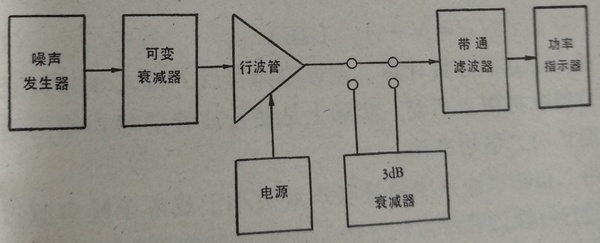
\includegraphics[width=0.6\linewidth]{figure/ch11-7}
	\caption{用二倍功率法测量噪声系数的原理方框图}
	\label{ch11-7}
\end{figure}

在微波波段,噪声源一般采用插入波导中的气体放电噪声管,当它点燃时,产生噪声并有较大的输出。衡量它输出噪声的大小,用过剩噪声比$ N $:

\begin{equation} \label{eq:11-6}
	N = \frac{KT_e\Delta f -KT_0\Delta f}{KT_0\Delta f} = \frac{T_e - T_0}{T_0}
\end{equation}

式中:

$ T_0 $—室温(K)


$ T_e $—气体放电管的等效噪声温度(K)


一般过剩噪声比也用分贝表示:
\begin{equation} \label{eq:11-7}
	N = 10\lg \frac{T_e - T_0}{T_0}\,\textrm{dB}
\end{equation}


功率指示器原则上应该用带有滤波器(带宽为$ \Delta f $)的功率计,但由于被测噪声功率很小,功率计不够灵敏,所以常常使用带有平方律检波器的超外差接收机,并在接收机前加一个带通滤波器。


在测量时,先不点燃噪声发生器,使被测行波管通过带通滤波器与接收机相连接,记下此时接收机的指示$ d_1 $;然后点燃噪声发生器,在行波管与接收机的滤波器之间接入一个3分贝的衰减器,调节可变衰减器,使接收机指示仍为$ d_1 $,记下此时可变衰减器的衰减量$ A$(dB),则被测行波管的噪声系数$ NF $(dB)为:
\begin{equation} \label{eq:11-8}
	NF = N - A \,\textrm{(dB)}
\end{equation}
式中$ N $、$ A $都以分贝计算。点燃噪声管后,接入3分贝衰减器而维持接收机指示不变,实际上是使行波管的噪声输出增加一倍,所以叫二倍功率法。


用二倍功率法只能测量噪声系数小于或等于噪声源过剩噪声比的行波管。若$ N $为18分贝,则用该法所能测量的噪声系数最大值也是18分贝。在微波接力通信中,行波管作为末级功率放大器,一般是中小功率行波管,其噪声系数比较大,约为24\textasciitilde28分贝,如果噪声源的过剩噪声比还是18分贝,则二倍功率法就不适用了


为了测量大噪声系数,应当采用自动噪声系数测试仪,它能测量大的噪声系数,而且还能自动显示噪声系数的大小,无需象二倍功率法那样,在测量过程中要读两次数。关于噪声系数测试仪的原理,因超出本书范围,不再介绍。仅给出如图\ref{ch11-8}所示的用自动噪声系数测试仪测量噪声系数的原理方框图。

\begin{figure}[phtb]
	\centering
	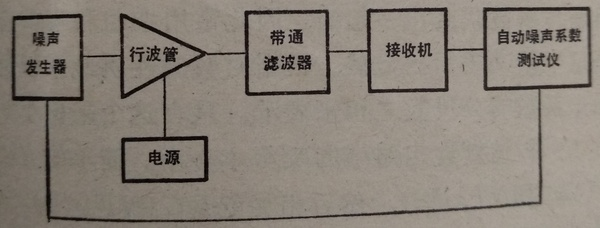
\includegraphics[width=0.6\linewidth]{figure/ch11-8}
	\caption{自动噪声系数测试仪测量噪声系数原理方框图}
	\label{ch11-8}
\end{figure}

噪声发生器未启动时,由\eqref{eq:11-4}可知行波管输出噪声为:
\begin{equation*} 
	N_2 = GNFKT_0\Delta f
\end{equation*}


当噪声发生器启动后,行波管输出噪声为:

\begin{equation} \label{eq:11-9}
	N_2' = GNFKT_0\Delta f + N\cdot GKT_0\Delta f
\end{equation}

所以:\[ \frac{N_2'}{N_2} = \frac{NF + N}{NF}  \]

即:
\begin{equation} \label{eq:11-10}
	NF = \frac{N}{\frac{N_2'}{N_2} -1}
\end{equation}
自动噪声系数测试仪使噪声发生器周期性地启动和灭火(如每秒钟500次),测出$ N_2'/N_2 $,再按照相应的$ NF $刻出刻度来。这样,人们从噪声系数测试仪上就可直接读出噪声系数$ NF $来。

\subsection[基带热噪声]{基带\footnote{基带:信号在调制以前所占有的频带,如960路电话通信的基带频率为60—4028千赫。}热噪声}

在调频制接力通信系统中,行波管的噪声系数在电路中所起的作用是与增益联系在一起的,因此常用增益和噪声系数两者的乘积这个量来表示。显然,根据对数的性质此乘积也可用增益与噪声系数的分贝数之和来表示。只有这个乘积小(分贝数之和小),行波管在电路中的噪声才会小。简单的方法是分别测量$ G $(dB)和$ NF $(dB),然后相加就是$ G\cdot NF $(dB)。

在测量噪声系数时,我们研究的是在带宽$ \Delta f $以内的行波管总的噪声功率,而不管噪声功率在$ \Delta f $以内是如何分配的。但是,当行波管内存在等离子振荡\footnote{行波管内的等离子振荡是由管内真空度的降低引起的。当管内真空度降低时,气体分子密度就要增大。这些气体分子在电子注的轰击下纷纷电离,变成正离子,它们在一定的条件下会产生所谓“等离子振荡”,其振荡频率(与正离子密度有关)通常都在基带内,振荡幅度很大,因此是十分有害的。},并且振荡频率在基带以内时,则在$ \Delta f $以内的某些频率上就会出现明显的噪声峰,它影响通信,严重时会使几百个话路的信噪比变坏。行波管在基带以内的噪声叫基带噪声,它实际上表示了行波管的噪声在基带以内的分布,如图\ref{ch11-9}所示。

\begin{figure}[phtb]
	\centering
	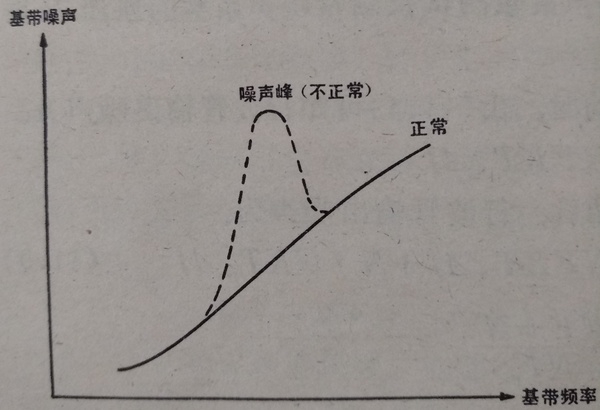
\includegraphics[width=0.6\linewidth]{figure/ch11-9}
	\caption{基带噪声}
	\label{ch11-9}
\end{figure}

测量基带噪声最简单的办法是在微波收发信机上进行,如图\ref{ch11-10}所示。我们让调制器只送出载频信号(不加调制信号),经过被测系统后,解调器收到的都是噪声,这时,用选频电平表在基带以内从低频向高频测量噪声电平曲线,不应出现明显的噪声峰。


图\ref{ch11-10}中,虚线方框\uppercase\expandafter{\romannumeral1}表示微波收发信机的发信部分(不包括行波管),\uppercase\expandafter{\romannumeral2}表示收信部分。这种方法测量出来的噪声,实际上是收发信两部分和行波管、调制器、解调器等几部分基带热噪声的总和。我们知道,在不加重、不加权的情况下以960路电话通信为例,在基带频率为4028千赫时一个话路测得的热噪声功率为200多微微瓦,而行波管仅占几微微瓦。因此,用这样的方法不能测出行波管的基带噪声电平。但是旦管内出现了离子振荡,行波管在某一基带频率附近的热噪声就立即升到几百、几千、甚至几万微微瓦,致使几十、几百个话路不能通话,此时便可用选频表测试出来。所以,这种方法只能检查行波管内有无噪声峰。

\begin{figure}[phtb]
	\centering
	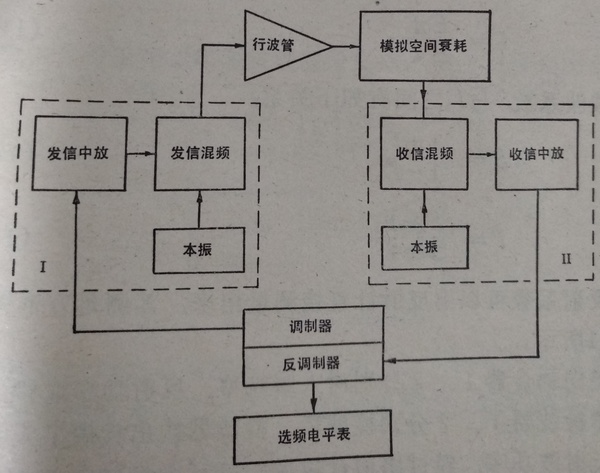
\includegraphics[width=0.6\linewidth]{figure/ch11-10}
	\caption{测量行波管的基带噪声原理方框图}
	\label{ch11-10}
\end{figure}

如何得到行波管的噪声功率数值呢?好在行波管还有噪声系数这一指标,在没有噪声峰的前提下,可以通过噪声系数和增益计算行波管的基带噪声功率。也可用专用的仪表直接测量行波管的基带噪声功率。由于设备复杂、限于本书篇幅,这里就不再介绍了。

\section{驻波系数}
行波管输入端和输出端的输能装置,不论它是同轴电缆还是波导管,都希望与传输线很好地匹配,即反射越小越好。但是,实际上总有一定的反射。衡量这个反射大小的量是反射系数$ \varGamma $或驻波系数$ S $(又叫驻波比)


反射系数$ \varGamma $指的是传输线上信号的反射波电场强度与入射波电场强度之比,即:
\begin{equation} \label{eq:11-11}
	\varGamma = \frac{E_\textrm{反}}{E_\textrm{入}}
\end{equation}

驻波系数$ S $与$ \varGamma $之间有如下关系:
\begin{equation} \label{eq:11-12}
S = \frac{1 + \varGamma}{1-\varGamma}
\end{equation}


或:
\begin{equation} \label{eq:11-13}
	\varGamma = \frac{S-1}{S+1}
\end{equation}

反射系数可以用反射计直接测量出来,其测量方框图如图\ref{ch11-11}所示。

\begin{figure}[phtb]
	\centering
	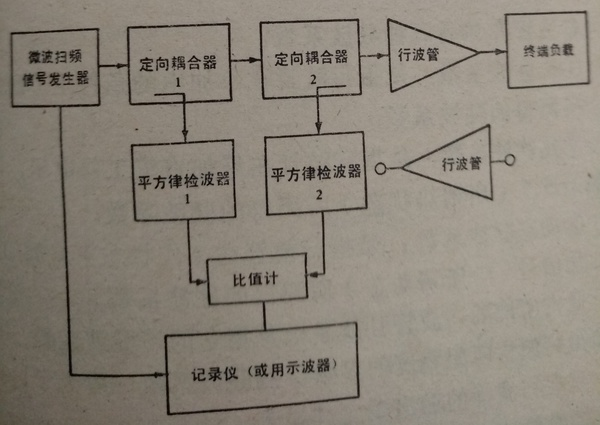
\includegraphics[width=0.6\linewidth]{figure/ch11-11}
	\caption{用反射计测量反射系数原理方框图}
	\label{ch11-11}
\end{figure}

定向耦合器1、2分别对入射功率、反射功率取样,经过平方律检波器1、2分别检波后,检波器输出代表了入射波功率和反射波功率,经过比值计以后,就可求得反射系数$ \varGamma $,或者在比值计上直接按$ S $刻出刻度。为了测量方便,用$ X-Y $记录仪(或示波器)可观察整个扫频范围内$ \varGamma $(或$ S $)的变化。

为了使测量准确,两个定向耦合器、两个检波器都要完全一样。微波扫频信号发生器的输出要稳幅,以保持入射波功率恒定。


驻波系数也可以用测量线测量出来,如图\ref{ch11-12}所示。

\begin{figure}[phtb]
	\centering
	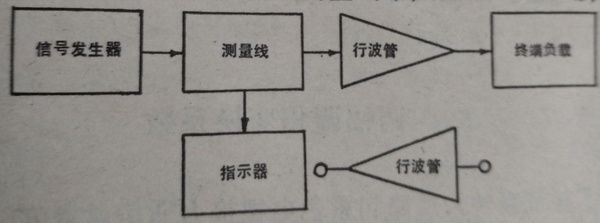
\includegraphics[width=0.6\linewidth]{figure/ch11-12}
	\caption{用测量线测量驻波系数原理方框图}
	\label{ch11-12}
\end{figure}

用测量线测出驻波的最大点指示$ D_{\textrm{max}} $、最小点指示$ D_{\textrm{min}}$,若测量线中检波器工作在平方律检波范围内,则驻波比为\footnote{所谓平方律检波是指当晶体的检波电流很小时,检波电流$ I $是和检波电压$ U $的平方成正比的$ I\propto U^2 $而测量线测得的检波电压$ U $又是与波导或同轴线内的电场大小$ E$成正比的。根据驻波系数的定义$ S = \frac{E_{\textrm{max}}}{E_\textrm{min}} $即可得$ S=\sqrt{\frac{D_\textrm{max}}{D_\textrm{min}}} $。}:

\begin{equation} \label{eq:11-14}
	S = \sqrt{\frac{D_\textrm{max}}{D_\textrm{min}}}
\end{equation}

行波管存在着三种驻波系数:

(1)冷驻波系数:是指行波管在不加电的条件下(所谓冷状态)所测得的驻波系数;


(2)热驻波系数:是指行波管在只加直流工作电压,不加信号的条件下(所谓热状态)所测得的驻波系数;


(3)动态驻波系数:是指行波管在工作状态下(加工作电压、加信号—所谓动态)所测得的驻波系数。


通常所说的行波管驻波系数是指它的冷驻波系数,用来作为衡量行波管匹配程度的参数。热驻波系数一般大于冷驻波系数,这在行波管的输出端尤其显著。


动态驻波系数的测量比较复杂,而且不常用。


在地面通信设备中,每一个行波管的工作带宽只有几十兆赫,因此,只要在此范围内把驻波系数调整到最佳就可以了。当然,如果在全频段内都不需要调整而能满足要求,那就更好。

\section{调幅调相变换系数}
为了保证微波大通路和彩色电视接力通信设备的传输质量,行波管还有调幅调相变换系数这一指标。它是指在给定的工作条件下,行波管的输入信号每改变1分贝,输出信号相位的变化度数,通常以$k_p $表示,单位是度/分贝。


图\ref{ch11-13}为行波管的输出功率$ P_\textrm{出} $、相位$ k_p $随输入功率的变化曲线。从曲线得知,为使$ k_p $小,方法之一是使输出功率小于饱和功率,并且输出功率越小,则$ k_p $越小。但是,这样做的缺点是使行波管工作时的效率降低了。

\begin{figure}[phtb]
	\centering
	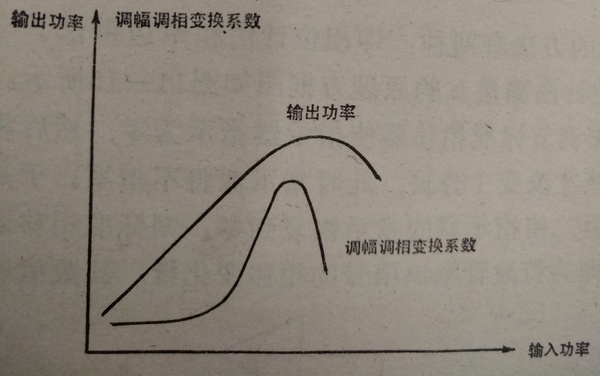
\includegraphics[width=0.6\linewidth]{figure/ch11-13}
	\caption{调幅调相变换系数、输出功率随着输入信号功率变化的曲线示意图}
	\label{ch11-13}
\end{figure}

方法之二是使行波管的螺旋线电压比同步电压略低(例如低50\textasciitilde100伏)——所谓偏同步使用。


图\ref{ch11-14}是$ k_p $、$ P_\textrm{出} $随螺旋线电压变化的曲线图。可见,在同步点$ k_p $不是最小值(图中$ a $点)。随着螺旋线电压的降低,$ k_p $也降低。偏同步以后,输出功率和工作效率虽然都有所降低,但却能使$ k_p $显著地获得改善。而输出功率的降低,比远离饱和点(方法一)降低的功率少得多。当然,降低$ k_p $的根本途径,是从管子设计上来改进。

\begin{figure}[phtb]
	\centering
	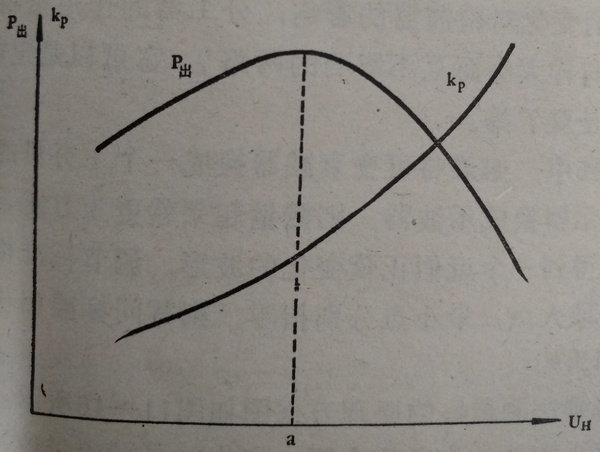
\includegraphics[width=0.6\linewidth]{figure/ch11-14}
	\caption{$ k_p $随螺旋线电压$ U_H $的变化}
	\label{ch11-14}
\end{figure}

测量$ k_p $的方法有两种:即相位计法和单边带法。


用相位计法测量$ k_p $的原理方框图如图\ref{ch11-15}所示。其测试方法是:先调节标准相移器使指示器指示为零,然后将可变衰减器的衰减量改变1分贝,此时指示器将不指零。于是再调节标准相移器,使指示器的指示恢复到零,则标准相移器相移的变化量,即为行波管输出信号的相移变化量,其数值就是$ k_p $。

图\ref{ch11-15}中,相位检波器采用和差法相位检波器,用以减小信号幅度的变化对检波器的影响;分工器的作用是将信号源的信号分为同样大小而互不影响的两路,它可以是定向耦合器,也可以是双$ T $等。

\begin{figure}[phtb]
	\centering
	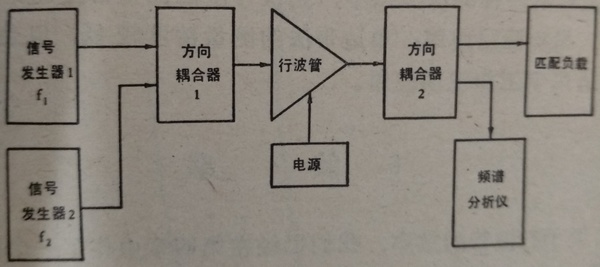
\includegraphics[width=0.6\linewidth]{figure/ch11-15}
	\caption{用相位计测量$ k_p $原理方框图}
	\label{ch11-15}
\end{figure}

图\ref{ch11-15}中,如果将可变衰减器换成一个1分贝的幅度调制器,将指示器换成示波器,则测量起来就更为方便。这时在示波器上可得到一个近似正弦变化的波形,调节标准相移器使此波形的最大点、最小点分别指零,则其间标准相移器相移的改变量即为$ k_p $。


用单边带法测量$ k_p $的原理方框图如图\ref{ch11-16}所示。借助于信号发生器1和2、方向耦合器1产生一个单边带信号,如图\ref{ch11-17}(左)所示。信号$ f_1 $和$ f_2 $的频率间隔很小(如1兆赫),幅度差约为20\textasciitilde30分贝。经过行波管以后,单边带信号变为不对称的双边带信号,如图\ref{ch11-17}(右)所示。测量双边带信号的幅度,就可以求出$ k_p $:

令:\begin{equation*}
	\begin{aligned}
	S_1^2 &= \frac{P_2}{P_1}\cdot \frac{P_{i1}}{P_{i2}}\\
	S_2^2 & = \frac{P_3}{P_1}\cdot\frac{P_{i1}}{P_{i2}}
	\end{aligned}
\end{equation*}
则
\begin{equation}\label{eq:11-15}
	k_p = 13.19\left[ S_1^2 - \frac{1}{4}\left( 1+S_1^2 - S_2^2 \right)^2 \right]^\frac{1}{2} \, {}^\circ/\textrm{dB}
\end{equation}
\begin{figure}[phtb]
	\centering
	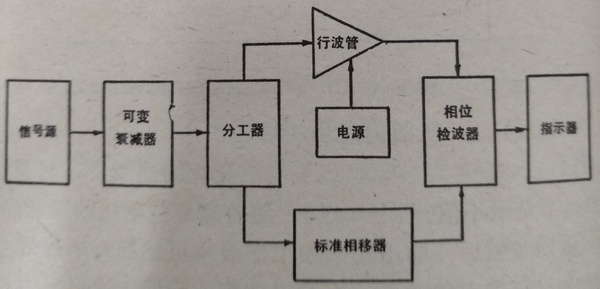
\includegraphics[width=0.6\linewidth]{figure/ch11-16}
	\caption{用单边带法测量$ k_p $原理方框图}
	\label{ch11-16}
\end{figure}

\begin{figure}[phtb]
	\centering
	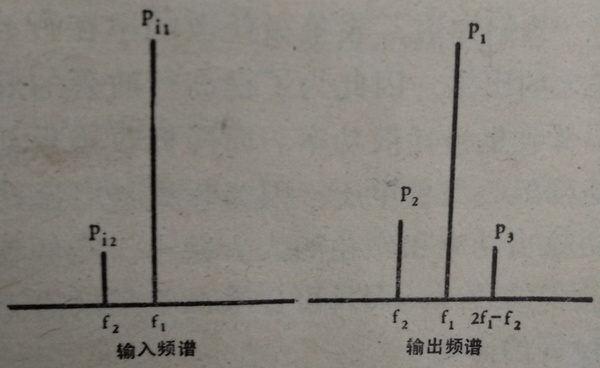
\includegraphics[width=0.6\linewidth]{figure/ch11-17}
	\caption{单边带法测量$ k_p的信号频谱 $}
	\label{ch11-17}
\end{figure}

为使测量和计算方便,常使$ P_{i1}/P_{i2} $为一定值(如$ 10\lg \frac{P_{i1}}{P_{i2}} = 30\textrm{dB} $),用频谱分析仪直接读取$ 10\lg\frac{P_2}{P_1} $和$ 10\lg\frac{P_3}{P_1} $,然后计算出$ S_1^2 $和$ S_2^2 $,即可进一步求出$ k_p $的数值。

上述的两种测量方法中,相位计法的测量精度较高,适用于工厂和实验室使用;单边带法的测量精度较低,但测量方便,适用于工作现场使用。

\section{效率}
关于行波管的效率,我们已经在第\ref{ch4}章中作了一个简单的介绍。这里想着重谈一下利用降压收集极来提高行波管的效率问题。


我们知道,收集极耗散功率在行波管的总耗散功率中占有很大的比重,因此为了提高行波管的效率,最有效的办法就是降低收集极耗散功率。而降低收集极耗散功率的最有效措施就是降低收集极电压,因为收集极电流是不能降低的,否则将导致输出功率和增益的大大减小。降低收集极电压不但能提高行波管的效率,而且可以降低收集极的工作温度因而可以延长行波管的寿命。


收集极电压降低以后将出现一些新的问题,如二次电子问题、动态散焦问题等,因此不能无限制地降低收集极电压。我们通常可以画出行波管的$ I_H\textasciitilde U_C $特性曲线,来表示该行波管的降压特性,如图\ref{ch11-18}所示。由图可见行波管的动态降压特性(高频输出功率$ P= $额定值时的降压特性)要比静态降压特性($ P=0 $时的降压特性)差,这是因为当行波管内有高频信号输入时,高频信号将与电子注发生作用,使电子流群聚。在群聚电子流中,电子的速度迅速向两极分化:快电子越来越快,慢电子越来越慢。这些慢电子在穿出螺旋线以后,如果遇到较强的减速场(收集极电压越低,收集极和螺旋线之间的减速场就越强)就很容易返转到螺旋线中并打到螺旋线上,使螺旋线电流增大。这就是行波管内有高频信号输入时收集极降压特性变差的原因。高频输出功率$ P $越大,说明电子流群聚越厉害,电子的两极分化越严重,慢电子越多,因而其降压特性就越差。

\begin{figure}[phtb]
	\centering
	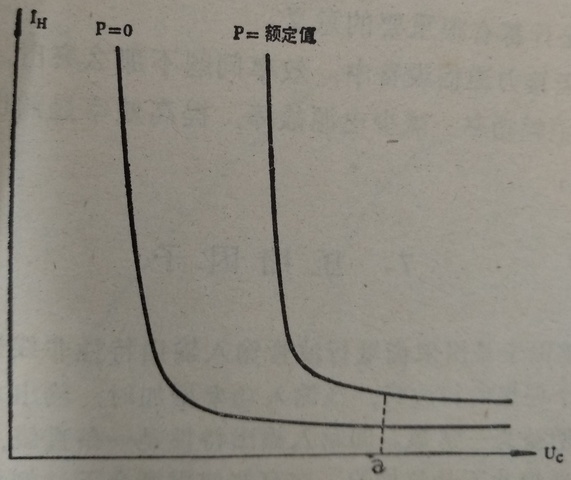
\includegraphics[width=0.6\linewidth]{figure/ch11-18}
	\caption{收集极降压特性}
	\label{ch11-18}
\end{figure}

我们常常根据降压特性来选择合理的收集极工作电压。一般应选择在降压特性曲线中离拐弯处较远一点的地方,如图\ref{ch11-18}中的$ a $点。这样,工作起来留有一定的余地,不会出现$ I_H $突然增大的情况。


为了改善行波管的收集极降压特性以提高行波管的效率,人们在收集极的结构上下了很大的功夫,制成了多级降压收集极,把行波管的效率提高到40\%以上,限于篇幅,我们这里就不多介绍了。


对通信卫星上所用的行波管来讲,效率有特别重要的意义,它是卫星行波管的主要指标之一。因为,效率提高后,行波管电源的重量和体积便可相应减小,而俄们知道,卫星重量每减轻1公斤都有很重要的意义。


在地面接力通信设备中,效率问题不那么突出。不过为了降低电源消耗功率,减少电源故障,提高效率显然也是一个重要的问题。
\section{压缩因子}
压缩因子是用来衡量行波管输入输出特性非线性的一个参量。一个理想的行波管,当输入功率增加时,输出功率线性地增加,增益为一常数。即输入输出特性是一条直线,但是,实际的行波管并不是这样的。在有些使用场合下,例如当调幅波通过行波管放大时,为了保证传输质量,行波管的幅度非线性问题就非常重要。这就需要用到压缩因子这个参量了。那么压缩因子是什么东西呢?我们把它的定义写在下面:
\begin{equation} \label{eq:11-16}
	C = \left( 1-\frac{\frac{\Delta P_\textrm{出}}{P_\textrm{出}}}{\frac{\Delta P_\textrm{入}}{P_\textrm{入}}} \right)\times 100\%
\end{equation}

注意,这里$ C $不是行波管的增益参量,不要把两者搞混了。式中$ \Delta P_\textrm{出} $为输入功率变化$ \Delta P_\textrm{入} $时输出功率的变化。如果用分贝表示$ \Delta P_\textrm{入} $和$ \Delta P_\textrm{出} $,那么,压缩因子$ C $可以写成:
\begin{equation} \label{eq:11-17}
	C = \left( 1 - \frac{\Delta P_\textrm{出}}{P_\textrm{入}} \right)\times 100\%
\end{equation}


\begin{figure}[phtb]
	\centering
	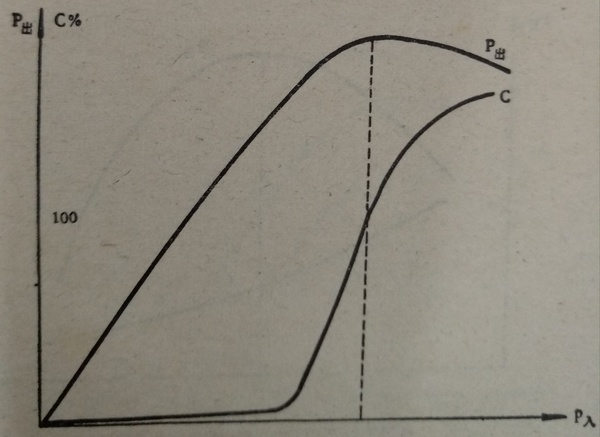
\includegraphics[width=0.6\linewidth]{figure/ch11-19}
	\caption{压缩因子随$ P_\textrm{入} $变化}
	\label{ch11-19}
\end{figure}
我们在图\ref{ch11-19}中画出了实际的行波管的输入输出特性及相对应的压缩因子曲线。由图可见:

(1)在小信号状态下行波管的输入输出特性是线性的,因而其增益为一常数,压缩因子$ C $等于零。


(2)随着输入功率的增加,输出功率并不是线性地增加,也就是说输入输出特性变成非线性了,一般说来,用分贝表示的$ \Delta P_\textrm{出} $要比$ \Delta P_\textrm{入} $小,因此,$ 0< C < 100\% $


(3)当输出功率饱和时,在饱和点附近,$ \Delta P_\textrm{入} $所引起的$ \Delta P_\textrm{出} $趋于零,因此$ C = 100\% $。


(4)当我们再继续增大输入功率时,将会发现输出功率不但不增加反而有所减小。这就是所谓过饱和区。此时,$ \Delta P_\textrm{入}>0 $时$ \Delta P_\textrm{出} < 0$,因此$ C $将大于100\%。


我们还发现:压缩因子和螺旋线电压也有关系。图\ref{ch11-20}中画出了对应的$ P_\textrm{出}\textasciitilde U_H$曲线即同步特性曲线。可见,当$ U_H $高于同步电压($ a $点)时,$ C $变好;$ U_H $低于同步电压时$ C $变坏。因此,如果考虑到幅度非线性,那么,$ U_H $高于同步电压运用比较好;如果考虑到相位非线性(调幅调相变换),那么,$ U_H $低于同步电压运用比较好。可见,$ C $和$ k_p $两者是矛盾的。我们必须针对使用要求来选择工作状态。

\begin{figure}[phtb]
	\centering
	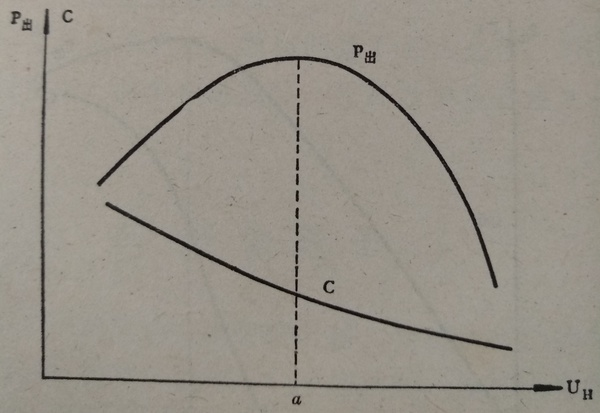
\includegraphics[width=0.6\linewidth]{figure/ch11-20}
	\caption{压缩因子和螺旋线电压关系曲线}
	\label{ch11-20}
\end{figure}

$ C $的测试较为简单,可先测出输入输出特性曲线,然后利用\eqref{eq:11-16}式算出不同输入功率时的$ C $,即可得到$ C\textasciitilde P_\textrm{入} $关系曲线。

\section{关于谐波}
当行波管输入一个单频(频率为$ f $)的高频信号时,在输出端除了得到该频率的放大信号以外,还常常可以得到它的高次谐波(例如$ 2f $、$ 3f $、$ 4f $……)信号。其中,通常以二次谐波影响较大。当输入功率增大(即更接近饱和)时,谐波分量也随之增大。我们常用谐波分量低于基波分量的分贝数来表示谐波分量的大小,并画于图\ref{ch11-21}中。由图可见,在饱和及过饱和状态下,二次谐波功率可以等于甚至大于基波功率。所以,为了减小谐波功率,除了在行波管设计上考虑以外,使用时,应尽可能工作在线性区。
\begin{figure}[phtb]
	\centering
	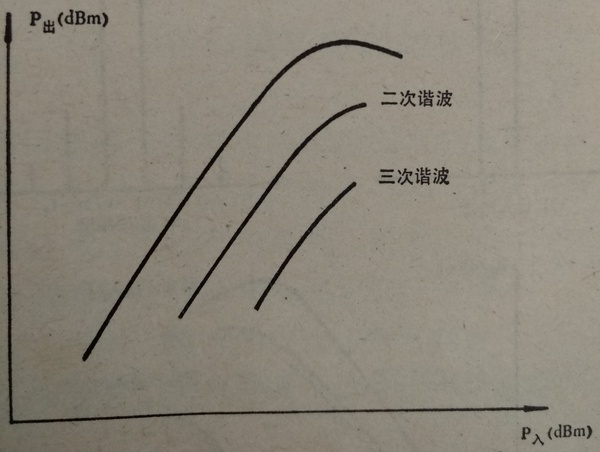
\includegraphics[width=0.6\linewidth]{figure/ch11-21}
	\caption{谐波功率曲线}
	\label{ch11-21}
\end{figure}
\section{互调失真}
在有些场合下,我们需要把几个频率的信号同时送入行波管中放大,此时,由于行波管的非线性效应,在输出端将出现其它分量的信号,这是我们不希望的。举个例子,若输入信号频率为$ f_1 $、$ f_2 $。则输出端除了$ f_1 $和$ f_2 $的信号以外,还有频率为$ mf_1\pm nf_2 $的信号($ m $、$ n $为正整数),这个现象称为互调制失真。我们用$ (m+n) $的数值来称呼它们的阶数,如$ 2f_1\pm f_2 $、$ f_1\pm 2f_2 $,就称为三阶互调制,$ 3f_1 \pm 2f_2 $、$ 2f_1 \pm 3f_2 $为五阶互调制等等。通常,$ (mf_1 -nf_2)$将落入接收机的通带内,因此对我们的工作影响较大,特别是三阶互调制影响最大,往往是我们研究的重点。图\ref{ch11-22}(a)画出了输入频谱,图\ref{ch11-22}(b)画出了输出频谱,图\ref{ch11-22}(c)画出了互调制分量随输入功率的变化。可见,输入功率越大(即越接近饱和),由于此时非线性现象严重,所以互调制分量也越大。
\begin{figure}[phtb]
	\centering
	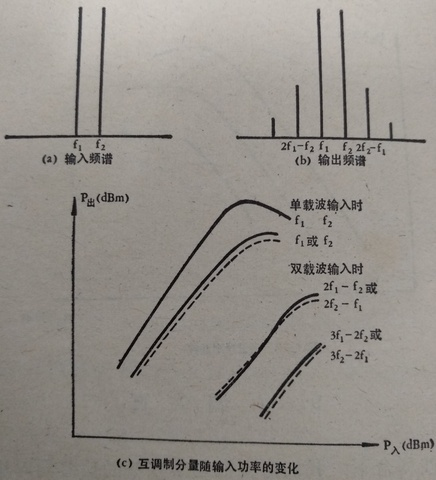
\includegraphics[width=0.6\linewidth]{figure/ch11-22}
	\caption{行波管的互调制失真}
	\label{ch11-22}
\end{figure}

测量互调制失真的方法是将等幅双载波信号送入行波管,然后测出输出端的$ (2f_1-f_2) $、$ (f_1-2f_2) $分量和载波信号$ f_1 $(或$ f_2 $),通常用互调分量比载波信号小的分贝数来表示互调制分量的大小,如图\ref{ch11-22}(c)所示。


测量谐波和互调制分量最简单的方法是用频谱分析仪,其原理方框图同图\ref{ch11-16}。


在多载波运用时,其中一个载波的幅度或相位的变化会引起另一些载波的幅度和相位的变化,这叫做交叉调制。它也有一系列的参数和专门的测试方法,由于比较复杂,在这里就不作介绍了。

\section{对行波管电源的要求}
除灯丝电压以外,行波管各极电压均为直流。灯丝电压可为直流或交流。有的行波管其灯丝有一端与阴极共用,此时,交流灯丝电压会通过阴极产生影响,以至在基带以内出现干扰。所以,这样的行波管最好用直流灯丝电压。


由于各极电压需采用直流电压,因此就有一个纹波值和稳定度的问题。下面我们就来看看各极电压对纹波值和稳定度的要求。


先说收集极电压,收集极只起收集工作完毕电子的作用,但决定收集极工作电压时需考虑效率、二次电子返转、动态散焦等因素,其综合表现就是收集极降压特性。通常我们选择收集极工作电压时往往留有一定的余地,因此,收集极电压的变化对于行波管的高频性能基本上没有影响。我们对收集极电压的要求也就可以比较低。当然,它的纹波和稳定度也不能太大,否则也会引起干扰,因为收集极电压是加在收集极和阴极之间的。


其次要谈到螺旋线电压,它的要求比较高。我们从同步特性可以看到,螺旋线电压偏离同步点不大的电压变化将会引起输出功率的可观变化。我们还讲过,螺旋线电压的变化还会引起压缩因子$ C $和调幅调相转换系数$ k_p $的变化。此外,螺旋线电压的变化还会引起相位的变化,这就是所谓相位灵敏度问题。通常,螺旋线电压每增加1\%,输出相位约减小几十度。既然螺旋线电压和这么多参量有关,因此对它的要求高一点也就不奇怪了。一般要求其纹波值为一百毫伏以下,稳定度为0.1\%。

至于阳极电压,由于它直接控制着收集极电流的大小,而收集极电流对高频性能有较大的影响。另一方面,阳极电压的变化也会引起输出端相位的变化,不过它的影响比螺旋线电压要小(阳极电压每增加1\%将使输出端相位增加约$ 5{}^\circ $),因此,对阳极电压纹波和稳定度的要求是介于收集极电压和螺旋线电压之间。


最后谈谈灯丝电压,一般要求其稳定度优于1\%。


为了保护行波管,通常在行波管电源中需安装螺旋线电流过荷保护装置,当螺旋线电流超过规定值时,继电器立刻动作,把全部高压切断。否则,螺旋线电流太大将烧坏螺旋线因而导致行波管失效。


在某些行波管电源中,还装有收集极温度监测装置,当收集极工作温度高于最高允许工作温度时,继电器就会立即动作,切断全部高压,以保护行波管。


在使用输出功率较大的行波管时,考虑到负载失配引起的反射功率也可能很大,它会从输出端反射回去烧坏行波管的集中衰减器。因此,需要在输出端安装监测负载反射功率的装置。当反射功率超过规定值时,就可立刻切断高压,保护行波管。但是,通常在微波接力通信设备中,行波管的输出功率并不大,因而不会产生上面的问题,也就没有必要安装监测装置了


我们知道,前面所说的各极电压都是相对于阴极而言的。但是,在使用时,为了安全起见,有时需要让螺旋线接地,有时需要让收集极接地。因此,在设计电源时,就需要考虑各极之间或各极与机壳之间的绝缘是否能满足要求。


通常,阳极电流是很小的(100微安以下),也就是说,阳极电源几乎可以不消耗功率。因此,我们常常可以从螺旋线电源上分出一部分电压或者在螺旋线电压上叠加一部分电压来作为阳极电压(视阳极电压与螺旋线电压何者高而定)这样就可以省去一组高压电源。它们的线路图示于图11-23和图11-24中。需要注意,在叠加式电路中,当调节螺旋线电压时阳极电压也随之变化,因此需同时调节阳极电压。

\begin{figure}[phtb]
	\centering
	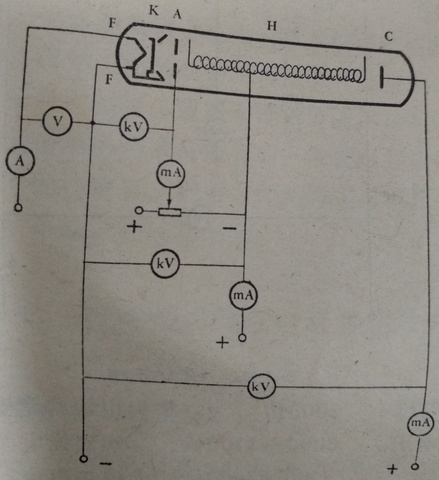
\includegraphics[width=0.52\linewidth]{figure/ch11-23}
	\caption{叠加式电源线路}
	\label{ch11-23}
\end{figure}

\begin{figure}[phtb]
	\centering
	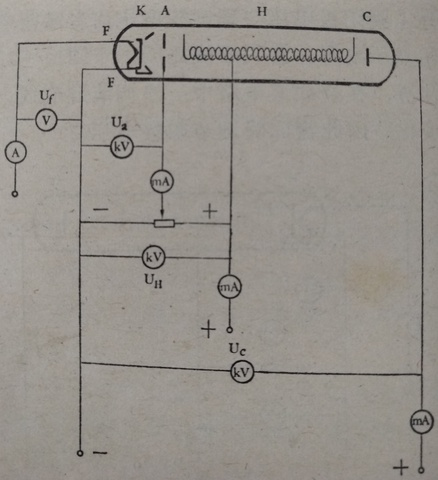
\includegraphics[width=0.52\linewidth]{figure/ch11-24}
	\caption{分压式电源线路}
	\label{ch11-24}
\end{figure}
\section{行波管参量举例}
为了使读者对于实际行波管的直流参量和高频参量的大小有一个大概的印象,我们来举一个例子说明一下。

某通信用行波管,其参量列举如表\ref{tab:11-1}所示。

\begin{table} 
	\caption{某通信行波管参量举例}
	\label{tab:11-1}
	\begin{tabular}{lrlr}
		\toprule
		\multicolumn{2}{c}{直流参量} & \multicolumn{2}{c}{高频参量}   \\ 
%		\cmidrule{1-2} 	\cmidrule{3-4}
	\midrule
		灯丝电压	& $ 6.3\pm 2\%伏 $ &工作频率范围$ f $  & 3.4\textasciitilde4.2千兆赫 \\ 
		灯丝电流	& $ <1 $安 & 饱和输出功率$ P $ & $ \ge 12 $瓦 \\ 
		灯丝最少预热时间	& 3分钟 & 饱和增益$ G $ & $ \ge 35 $分贝 \\ 
		收集极电压	&2000伏  & 噪声系数NF & $ \le 28 $分贝 \\ 
		收集极电流	& 35毫安 &调幅调相变换系数$ k_p $  & $ <3 $度/分贝 \\ 
		螺旋线电压	&3000\textasciitilde3300伏  & 增益斜率 & $ \le 0.01$分贝/兆赫  \\ 
		螺旋线电流	&  $ <2 $毫安&冷驻波比$ S $  &  $ \le 1.5 $\\ 
		阳极电压	& 3200\textasciitilde3600伏 &  &  \\
		阳极电流& $ <0.2 $毫安& & \\
		\bottomrule 
	\end{tabular} 
\end{table}



